\documentclass{exam}
\usepackage[utf8]{inputenc}
\usepackage{lmodern}
\usepackage{microtype}

% \usepackage[parfill]{parskip}
\usepackage[dvipsnames]{xcolor}
\usepackage{amsmath}
\usepackage{amsfonts}
\usepackage{amsthm}
\usepackage{siunitx}
\DeclareSIUnit\year{yr}
\DeclareSIUnit\foot{ft}
\DeclareSIUnit\litre{\liter}

\usepackage{skull}

\usepackage{pgfplots}
\usepgfplotslibrary{polar}
\pgfplotsset{compat=1.11}
\usepgfplotslibrary{statistics}
\usepackage{graphicx}
\usepackage{sidecap}
\sidecaptionvpos{figure}{c}
\usepackage{float}
\usepackage{gensymb}
\usepackage{tkz-euclide}
\usetkzobj{all}
\usepackage{commath}
\usepackage{hyperref}
\usepackage{enumitem}
\usepackage{wasysym}
\usepackage{multicol}
\usepackage{mathtools}
\usepackage{tcolorbox}
\usepackage{tabularx}
\usepackage[version=4]{mhchem}
\usepackage{changepage}
\usepackage{listings}
\lstset{basicstyle=\ttfamily\linespread{0.8}\small}

\renewcommand*{\thefootnote}{\fnsymbol{footnote}}

\newtheorem*{thm}{Theorem}
\newtheorem*{iden}{Identity}
\newtheorem*{lemma}{Lemma}
\newtheorem{obs}{Observation}
\theoremstyle{definition}
\newtheorem*{defn}{Definition}
\newtheorem*{ex}{Example}
\newtheorem{con}{Construction}
\newtheorem*{alg}{Algorithm}

\newtheoremstyle{break}
  {\topsep}{\topsep}%
  {\itshape}{}%
  {\bfseries}{}%
  {\newline}{}%
\theoremstyle{break}
\newtheorem*{bthm}{Theorem}

% russian integral
\usepackage{scalerel}
\DeclareMathOperator*{\rint}{\scalerel*{\rotatebox{17}{$\!\int\!$}}{\int}}

% \DeclareMathOperator*{\rint}{\int}

\pgfplotsset{vasymptote/.style={
    before end axis/.append code={
        \draw[densely dashed] ({rel axis cs:0,0} -| {axis cs:#1,0})
        -- ({rel axis cs:0,1} -| {axis cs:#1,0});
    }
}}

% \pointsinrightmargin
\boxedpoints
\pointname{}

\newcommand{\questioA}{\question[\texttt{\textbf{\color{Cerulean} A}}]}
\newcommand{\questioM}{\question[\texttt{\textbf{\color{PineGreen} M}}]}
\newcommand{\questioE}{\question[\texttt{\textbf{\color{WildStrawberry} E}}]}
\newcommand{\questioS}{\question[\texttt{\textbf{\color{Goldenrod} S}}]}
\newcommand{\questioO}{\question[\texttt{\textbf{\color{BurntOrange} O}}]}

\newcommand{\parA}{\part[\texttt{\textbf{\color{Cerulean} A}}]}
\newcommand{\parM}{\part[\texttt{\textbf{\color{PineGreen} M}}]}
\newcommand{\parE}{\part[\texttt{\textbf{\color{WildStrawberry} E}}]}
\newcommand{\parS}{\part[\texttt{\textbf{\color{Goldenrod} S}}]}
\newcommand{\parO}{\part[\texttt{\textbf{\color{BurntOrange} O}}]}

\newcommand{\subparA}{\subpart[\texttt{\textbf{\color{Cerulean} A}}]}
\newcommand{\subparM}{\subpart[\texttt{\textbf{\color{PineGreen} M}}]}
\newcommand{\subparE}{\subpart[\texttt{\textbf{\color{WildStrawberry} E}}]}
\newcommand{\subparS}{\subpart[\texttt{\textbf{\color{Goldenrod} S}}]}
\newcommand{\subparO}{\subpart[\texttt{\textbf{\color{BurntOrange} O}}]}

\newcommand{\mainHeader}[2]{\section*{NCEA Level 2 Mathematics\\#1. #2}}
\newcommand{\mainHeaderHw}[2]{\section*{NCEA Level 2 Mathematics (Homework)\\#1. #2}}
\newcommand{\seealso}[1]{\begin{center}\emph{See also #1.}\end{center}}
\newcommand{\drills}[1]{\begin{center}\emph{Drill problems: #1.}\end{center}}
\newcommand{\basedon}[1]{\begin{center}\emph{Notes largely based on #1.}\end{center}}


\begin{document}

\mainHeaderHw{2}{Arcs and Sectors of Circles}
\subsection*{Reading}
\begin{center}
\begin{tcolorbox}[width=0.8\textwidth,colback={white},title={\textbf{Go and watch...}},colbacktitle=black,coltitle=white]
  \textcolor{black}{\url{https://www.youtube.com/watch?v=QncgmzH6yQU}}
\end{tcolorbox}
\end{center}

\begin{center}
\begin{tcolorbox}[width=0.8\textwidth,colback={white},title={\textbf{What's it good for?}},colbacktitle=MidnightBlue,coltitle=white]
  People use the geometry of circles for...
  \begin{itemize}
    \item Physics: physicists and engineers often want to model things that rotate, and proper definitions of rotational speed and acceleration
          require the use of the geometry of arc lengths and sector areas.
    \item Mathematics: the idea of a `limiting process', where we take sums of things that we let become infinitesimally small, is a fundamental
          idea that underpins entire branches of mathematics and allows us to formally define the concepts of area and volume, and enables us
          to better understand things which are continuous.
  \end{itemize}
\end{tcolorbox}
\end{center}

\begin{center}
  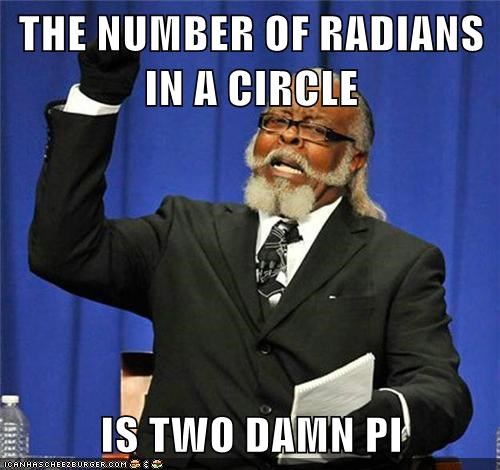
\includegraphics[width=0.5\textwidth]{trig1}
\end{center}

\subsection*{Questions}
\begin{questions}
  \question A car tire has diameter \SI{53}{\centi\metre}. A detector measures that a particular point on the tire tread
            rotates past 1061 times per second.
    \begin{parts}
      \part What speed is the car travelling at?
      \part Is this setup practical and/or useful? Explain.
    \end{parts}
  \question What is the radius of a circle such that the sector of area $ \frac{\pi}{3} $ has arc length $ \frac{\pi}{3} $?
\end{questions}

\end{document}
